Today, scale-free networks are of great importance. Many studies found them in the wild, regardless of natural or human-made networks, such as the World Wide Web \cite{Barabsi2000}, citation networks \cite{Wang2010}, and protein-protein interaction \cite{Nacher2009}.  See an example of a scale-free network in Figure \ref{fig:scale-free-network}

\begin{figure}[!htb]
    \centering
    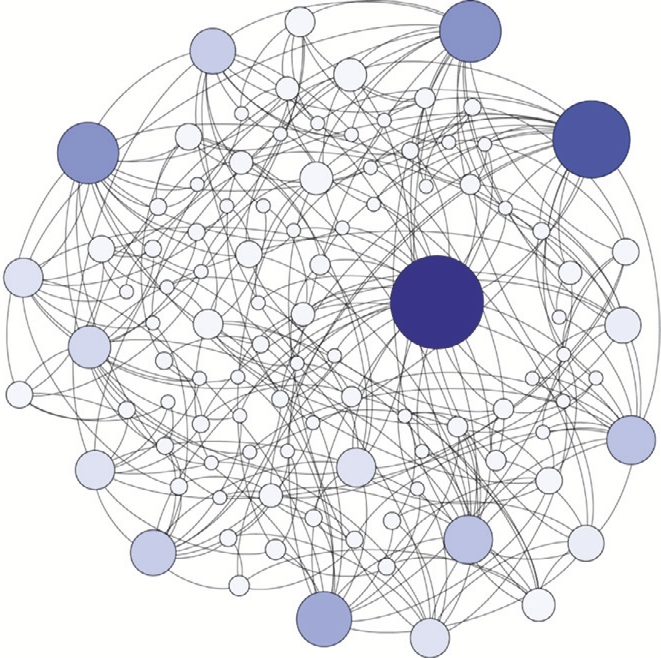
\includegraphics[width=0.5\textwidth]{figures/scale-free-network.jpg}
    \caption{A scale-free network in which very different nodes coexists with 100 nodes and average degree of $2.5$. The degree of each node is visually stressed by color and size. Figure extracted from \cite{Baronchelli2013}.}
    \label{fig:scale-free-network}
\end{figure}

Many studies use random, scale-free networks to better understand the underlying model of their own problem. The most widely used random model for scale-free networks was introduced by Albert-László Barabási and Réka Albert in 1999 \cite{Barabasi1999}. Their model uses two mechanics to achieve a scale-free network:
\begin{enumerate}[I]
    \item \textbf{Vertex Growth}. Growth means that the number of nodes in the network increases over time.
    \item \textbf{Preferential attachment}. This mechanism causes nodes with a higher degree to be more likely to acquire new links. This is because they have a greater capacity to attract links that are added to the network.
\end{enumerate}

During this report, we will examine how the different dynamic principles affect the random model. To do so, we will generate three random models: the classical Barabási-Albert model, the same model without preferential attachment, and finally, maintaining the preferential attachment and skipping the vertex growth. Then, we will analyse the degree distribution of the different models and the growth of vertex degree over time.

This document is structured in four different sections. Next, results are presented in Section \ref{sec:results}. Discussion and conclusions are covered in Section \ref{sec:discussion}, and finally some aspects of the methodology are presented in Section \ref{sec:methods}.